\chapter[Introdução]{Introdução}
\addcontentsline{toc}{chapter}{Introdução}

%Este documento apresenta considerações gerais e preliminares relacionadas 
%à redação de relatórios de Projeto de Graduação da Faculdade UnB Gama 
%(FGA). São abordados os diferentes aspectos sobre a estrutura do trabalho, 
%uso de programas de auxilio a edição, tiragem de cópias, encadernação, etc.

\section{Contextualização}

A preocupação e cuidados com a saúde sempre foram tópicos relevantes para a humanidade. Com a descoberta da eletricidade e estudo da biologia humana foram desenvolvidas tecnologias que unem ambas para prever, diagnosticar, tratar e monitorar o avanço de doenças. 

A evolução dessas tecnologias chegou ao ponto da criação de dispositivos \textit{wearables}(vestíveis). Esses dispositivos são criados de forma a serem usados no corpo do usuário como uma roupa. É uma tecnologia emergente que permite o monitoramento de sinais vitais no dia-a-dia, durante o trabalho, na prática de esporte e etc.\cite{site_wearebles}

Esse projeto visa o uso de monitoramento num ambiente hospitalar, onde será feita a captação do estado do paciente de forma mais confortável e constantemente sem precisar de contato físico. Isso é aplicável a pacientes que precisam de monitoramento constante e que estão em tratamento intensivo como UTI ou bebês em incubadoras.\cite{artigo_principal}

Dadas as considerações esse projeto propõe o desenvolvimento de uma \textit{tag RFID}, que será usada como sensor \textit{wearable} acompanhando o estado do paciente constantemente o paciente e funcionando de forma remota. Dado que a alimentação e transmissão das informações são feitas de maneira \textit{wireless} por rádio frequência como descrito na Fig. 
\ref{fig01}


\begin{figure}[h]
	\centering
	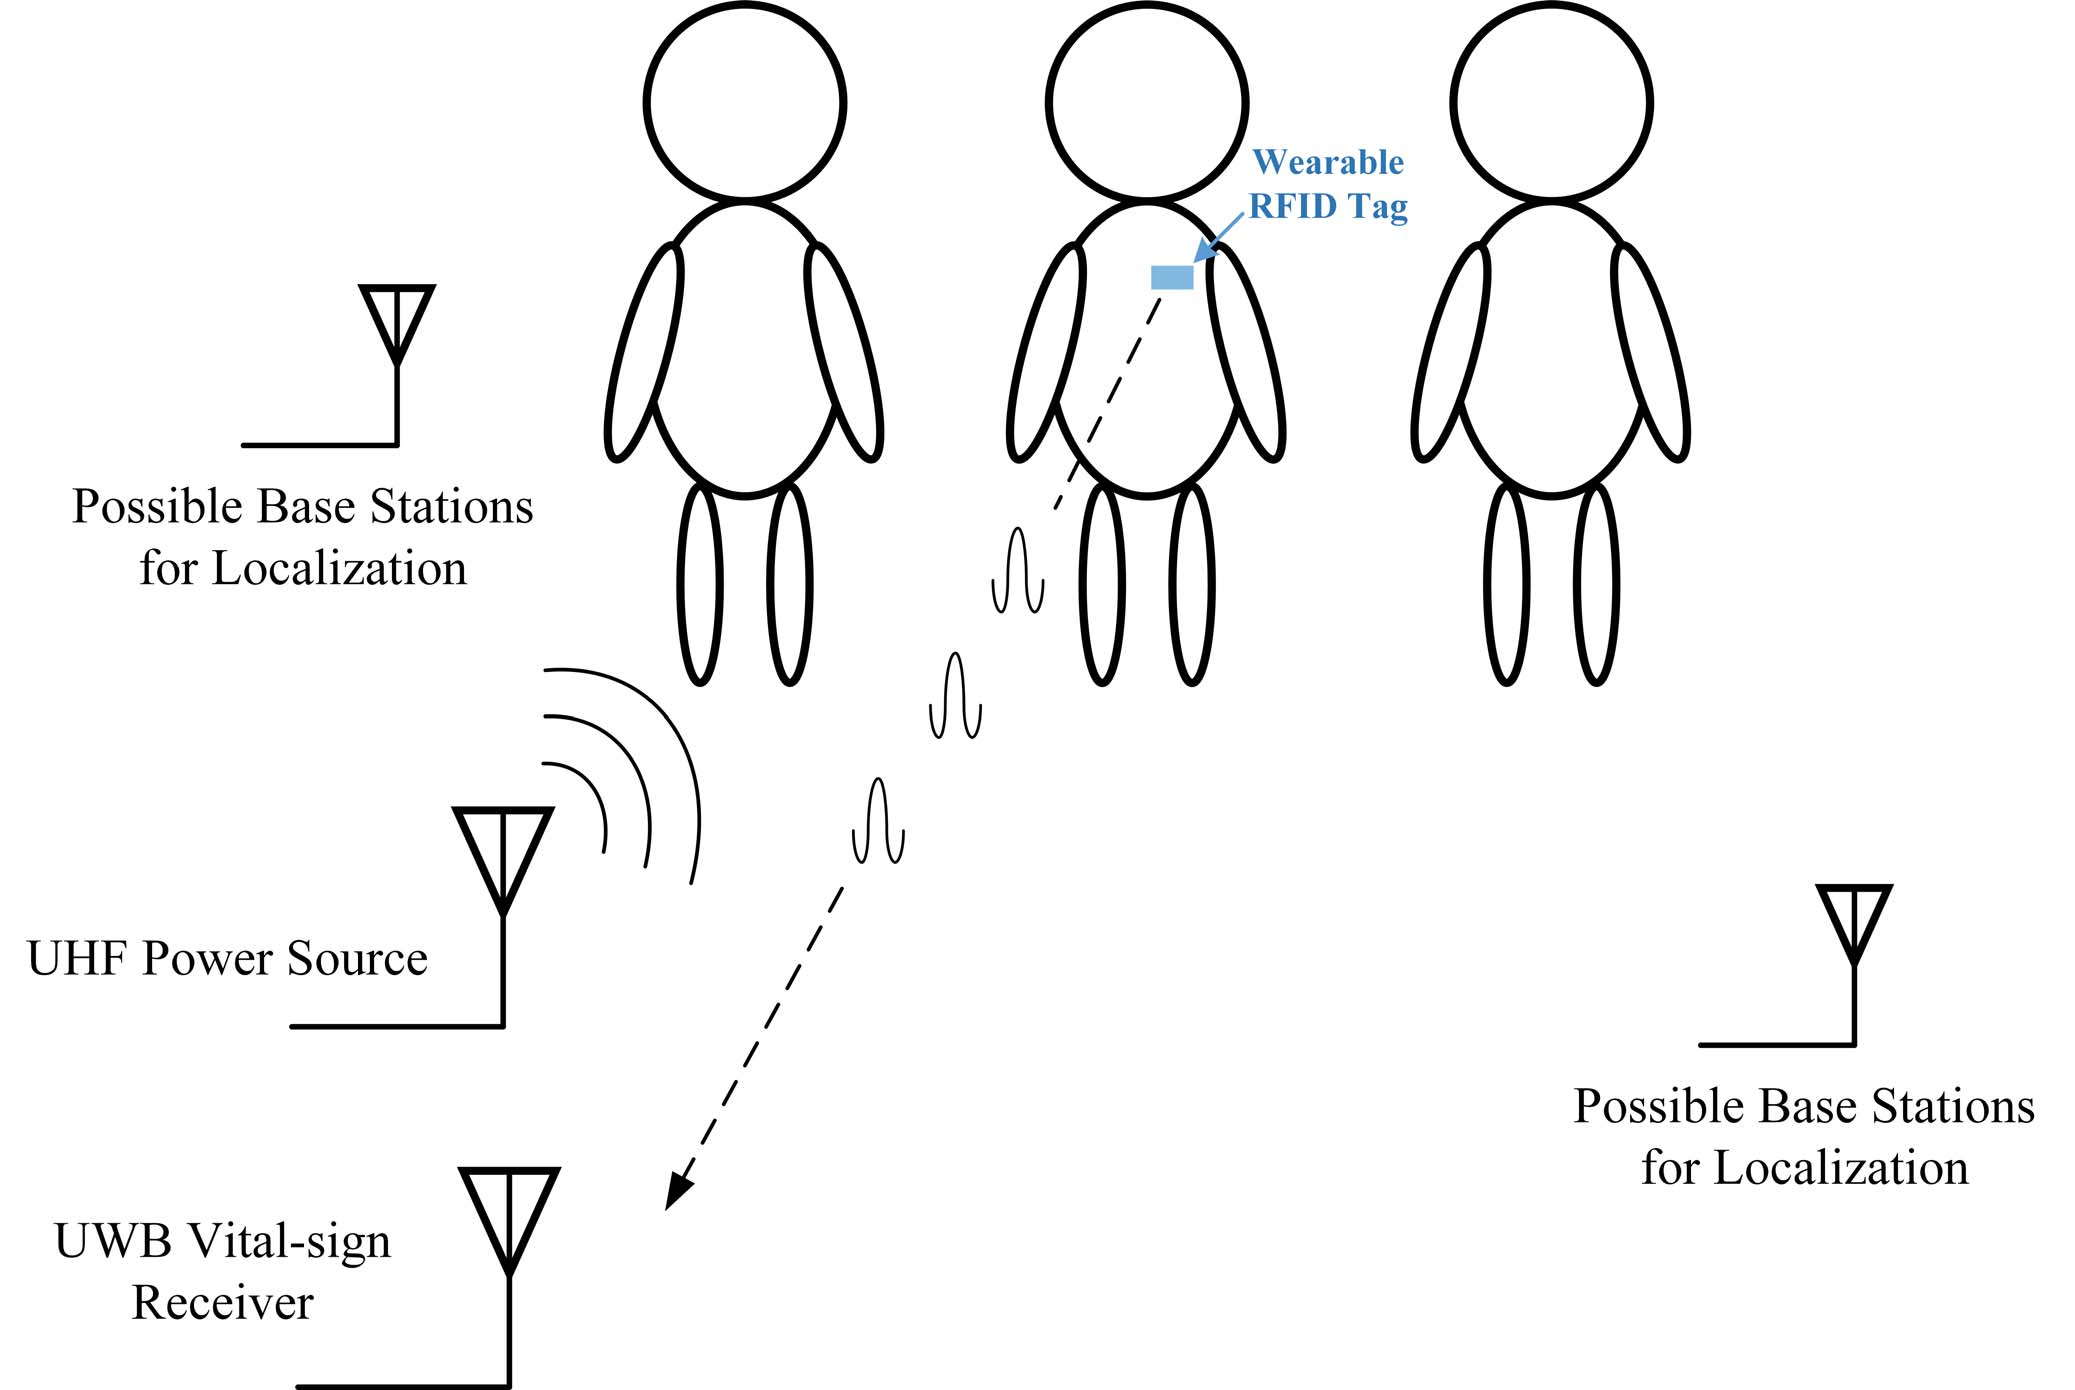
\includegraphics[width=0.6\textwidth]{figuras/rfid_tag.png}
	\caption{Ilustração da TAG RFID proposta para monitoramento remoto de sinais vitais. Fonte:\cite{artigo_principal} }
	\label{fig01}
\end{figure}

\subsection{Circuitos da \textit{TAG RFID}}

Na Fig. \ref{fig02} está a visão em \textit{Top Modulo} da \textit{TAG RFID}. Ela é composta por esses cinco subcircuitos representados em blocos sendo eles: Retificador, LDO, Tensão de referência (Bandgap), Conversor tensão frequência e o transmissor \textit{UWB}.

\subsubsection{Retificador}

O retificador é o circito responsável por alimentar o sistema, em resumo é um sistema de alimentação por indução. Ele capta o sinal de alimentação em rádio frequência e retifica tornando-o em DC para suprir a TAG com energia. 

\subsubsection{Tensão de Referência}

O circuito usado para tensão de referência foi o Bandgap. Ele vai gerar uma tensão de referência estável e resistente à variação de temperatura para ser usado no LDO.

\subsubsection{LDO}

O LDO é um regulador de tensão que vai ajustar uma voltagem menor para alimentar os outros subcircuitos que são o conversor tensão frequência e o transmissor \textit{UWB}.

\subsubsection{Conversor Tensão-Frequência}

Este componente é o objeto de discução dessa tese. Ele converte os sinais elétricos recebidos na tensão de entrada, que não é a alimentação, e converte num sinal de onda quadrada com a frequência equivalente à tensão de entrada.

\subsubsection{Transmissor \textit{UWB}}

Ele recebe o sinal produzido pelo conversor tensão frequência e o transmite o sinal que pode ser interceptado por outro equipamento.

\begin{figure}[htb]
	\centering
	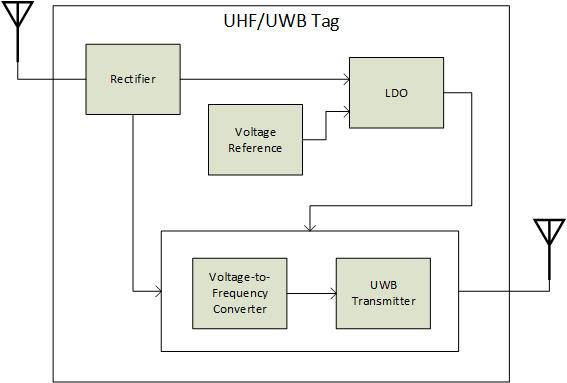
\includegraphics[width=0.6\textwidth]{figuras/Top.jpg}
	\caption{Visão do \textit{Top Module} da \textit{Tag RFID} desenvolvida no projeto. Fonte:\cite{artigo_tag_unb} }
	\label{fig02}
\end{figure}

\section{Objetivos}

 Para a execução do projeto será modelado o circuito de conversão tensão-frequência. Exibindo e explicando o funcionamento dos subsistemas que compõe esse circuito e a lógica aplicada nele começando pelas suas topologias e depois a simulação. Os blocos de subsistemas abordados são: conversor tensão corrente, integrador e sistema de controle.

\section{Organização}

Esse documento é organizado nas seguintes sessões:
\begin{itemize}
	\item \textbf{Sessão I Introdução}: Explicação das razões do projeto e contextualização
	\item \textbf{Sessão II Metodologia}: apresentação das metodologias aplicadas no projeto
	\item \textbf{Sessão III Conversor Tensão frequência}: exibição das topologias e explicação dos circuitos e blocos que compõe o conversor e como eles são relacionados.
	\item \textbf{Sessão IV Simulações}: Simulações dos circuitos feitas com a ferramenta de desenvolvimento Cadence Virtuoso
\end{itemize}




%Este template é uma adaptação do ABNTeX2\footnote{\url{https://github.com/abntex/abntex2/}}.
